\newgeometry{margin=0.1cm}

\begin{frame}{Residual of track parameters: $\Delta d_0$, $\Delta z_0$, $\Delta \phi_0$, $\Delta$cot$\theta$,$\Delta q/p_T$  ($\mu^{\pm}$~$p_T$ = 25 GeV)}
\begin{columns}
\column{0.45\textwidth}
\hskip-0.3cm
\includegraphics[width=1.\textwidth]{Thesis_6_3}
\vfill
\scalebox{0.5}{CERN-THESIS-2004-051 Fig.~6.3.}
\column{0.42\textwidth}
\hskip-0.3cm
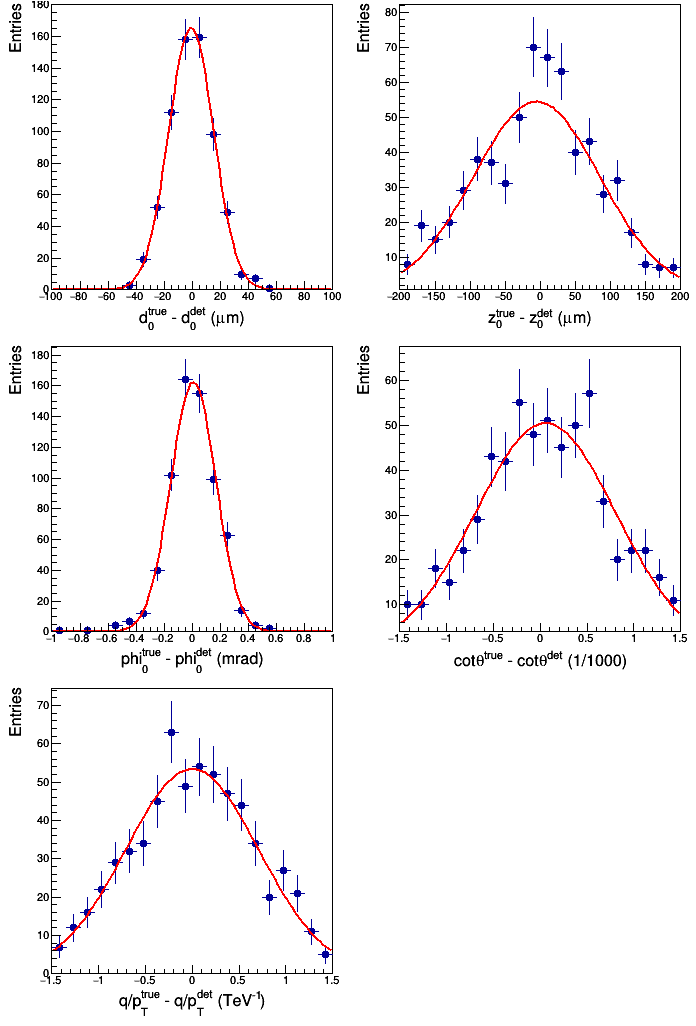
\includegraphics[width=1.\textwidth]{my_6_3_muons}
\vfill
\scalebox{0.5}{Example of smearing in a standalone G4 fast-sim, 20k muons , $\left|\eta\right|<5.5$}
\end{columns}
\end{frame}

\begin{frame}{Gaussian standard deviation $\sigma(p_T)$}
\begin{columns}
\column{0.45\textwidth}
\hskip-0.3cm
\includegraphics[width=1.\textwidth]{Thesis_6_5}
\vfill
\scalebox{0.5}{CERN-THESIS-2004-051 Fig.~6.5.}

\column{0.42\textwidth}
\hskip-0.3cm
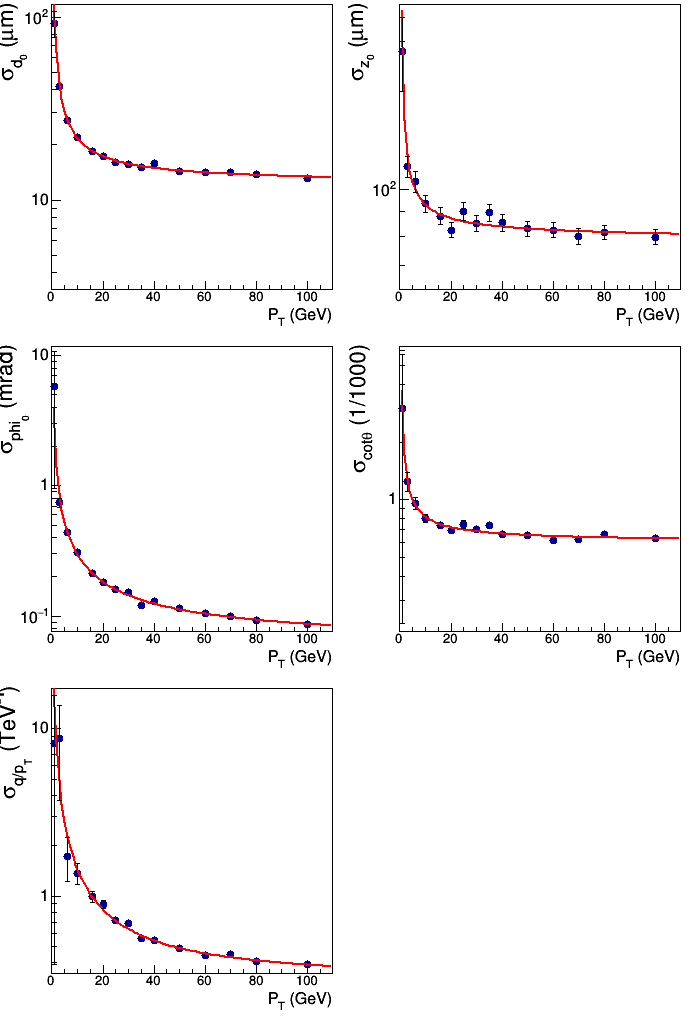
\includegraphics[width=1.\textwidth]{my_6_5_muons_log}
\vfill
\scalebox{0.5}{Example of smearing in a standalone G4 fast-sim, 20k muons , $\left|\eta\right|<5.5$}
\end{columns}
\onslide<2>
{
\begin{tikzpicture}[overlay,decoration=penciline,node distance = 0pt, outer sep = 0pt]
    tikzstyle{every node}=[font=\tiny]
% \draw[step=1cm,gray,very thin] (0,0) grid (6,6);
\node[text = violet] (t1) at (6,1.2) {\large scale on axes};
\node[text = violet, below = of t1] (t2) {\large is comparable};
%%%% d0
\node[Mark3] (qptM) at (1.15,6.1) {~~};
\node[text=violet, above = of qptM.west, yshift = 5pt, xshift=-12pt] {$10^{\textrm{-}3}~\mathrm{cm}$};
\node[Mark3] (qptMM) at (7.45,6.7) {~~};
\node[text=violet, above = of qptMM.east, yshift = 5pt, xshift=-15pt] {$10~\mathrm{\mu m}$};
%%%% z0
\node[Mark3] (thetaM) at (3.87,6.77) {~~};
\node[text=violet, above = of thetaM.north east, yshift = 1pt, xshift=16pt] {$10^{\textrm{-}2}~\mathrm{cm}$};
\node[Mark3] (thetaMM) at (10.07,6.8) {~~~};
\node[text=violet, above = of thetaMM.east, yshift = 0pt, xshift=15pt] {$10^2~\mathrm{\mu m}$};
%%%% phi0
\node[Mark3] (qptM) at (1.15,3.5) {~~};
\node[text=violet, above = of qptM.north west, yshift = 5pt, xshift=-12pt] {$10^{\textrm{-}4}~\mathrm{rad}$};
\node[Mark3] (qptMM) at (7.5,4.5) {~~};
\node[text=violet, above = of qptMM.north east, yshift = 5pt, xshift=15pt] {$10^{\textrm{-}1}~\mathrm{mrad}$};
%%%% cot theta
\node[Mark3] (thetaM) at (3.9,4.) {~~};
\node[text=violet, above = of thetaM.north east, yshift = 1pt, xshift=9pt] {$1$};
\node[Mark3] (thetaMM) at (10.1,4.45) {~~};
\node[text=violet, above = of thetaMM.east, yshift = 0pt, xshift=15pt] {$1\cdot\frac{1}{1000}$};
%%%% q/pt
\node[Mark3] (qptM) at (1.15,1.2) {~~};
\node[text=violet, above = of qptM.north west, yshift = 5pt, xshift=-12pt] {$10^{\textrm{-}3}~\mathrm{GeV}^{\textrm{-}1}$};
\node[Mark3] (qptMM) at (7.5,1.4) {~~};
\node[text=violet, above = of qptMM.north east, yshift = 5pt, xshift=-15pt] {$1~\mathrm{TeV}^{\textrm{-}1}$};
\end{tikzpicture}
}
\end{frame}


% \begin{frame}
% \begin{figure}[htbp]
% \begin{center}
% \scalebox{1}{\input{my_6_3_muons.tex}}
% \end{center}
% \end{figure}
% \end{frame}
\restoregeometry